\section{Theoretical Background}
\label{sec:literature}

This section provides an overview of artificial intelligence (AI), including hybrid intelligence, adaptive AI,
and how the use of such systems in enterprises can create a competitive advantage. Further, the editorial process 
is presented.

\subsection{AI and Hybrid Intelligence}

AI involves the creation of computer programs and algorithms that allow machines to replicate human cognition and behavior,
which includes the capabilities of perception, learning, reasoning, solving problems, and making decisions. AI can be broadly
subdivided into symbolic and sub-symbolic approaches, see e.g., \cite{eliasmithSymbolicSubsymbolic2006}. Symbolic approaches
involve the use of explicit symbols and rules to represent knowledge and reason in a way that is easily understood and explainable
by humans, while sub-symbolic (or \textit{connectionist}) approaches aim to learn complex patterns from vast amounts of data
using neural networks \citep{ilkouSymbolicVsSubsymbolic2020}. Hybrid AI refers to systems combining symbolic and sub-symbolic
approaches. Hybrid AI systems can be anywhere from loosely coupled to tightly integrated \citep{garcezNeurosymbolicAI3rd2023}.
Loosely coupled hybrid AI systems typically involve a human, which is also known as \textit{human in the loop} (HITL)
computing. In such systems the humans and AI work together towards common goals, augmenting the human intellect and
overcoming human limitations and cognitive biases \citep{akataResearchAgendaHybrid2020a}. This combination of human and machine
intelligence is known as \textit{hybrid intelligence}, \textit{augmented intelligence} or \textit{amplified intelligence}
\citep{schmidtAugmentingHumanIntellect2017,akataResearchAgendaHybrid2020a,zhouIntelligenceAugmentationBuilding2021}.
The tradition of hybrid intelligence can be traced back to Joseph Licklider's ``man-computer symbiosis'' and Douglas Engelbart's
vision of increasing human capabilities trough better and faster machine understanding \citep[and references cited therein]{schmidtAugmentingHumanIntellect2017}.
With the advanced and ubiquitous digital technologies now available, hybrid intelligent systems show the potential for improving
the outcomes of AI systems,  hence \textit{augmenting} rather than replacing human intelligence \citep{schmidtAugmentingHumanIntellect2017,
akataResearchAgendaHybrid2020a}. Further, \cite{kambhampatiChallengesHumanAwareAI2020} demanded that AI researchers build human-aware AI
systems that work synergistically with humans, including considering the human mental state, recognizing desires and intentions,
and providing proactive support to humans. In particular, AI researchers should aim at systems that show the capabilities of
\textit{explicability} (AI agents should show behavior that is expected by humans) and \textit{explainability} (AI agents -- 
if behaving unexpectedly -- should be able to provide an explanation) \citep{kambhampatiChallengesHumanAwareAI2020}.
Human-aware AI systems are designed to work alongside humans and must possess the ability to detect, comprehend, and respond
to a broad spectrum of human behavioral traits, including but not limited to \textit{``attention, motivation, emotion, creativity,
planning, or argumentation.''} \citep{kortelingHumanArtificialIntelligence2021}. As the cognitive abilities of human intelligence
are limited by the biological substrate as well as the biological and evolutionary origin of intelligence,
\cite{kortelingHumanArtificialIntelligence2021} argue the best approach to improve outcomes of AI system is to develop
human-aware AI systems that support human decision-making rather than pursuing the goal of Artificial General Intelligence (AGI).
This could mean that we continue to stick to \textit{narrow} AI models to develop human-aware AI systems for the foreseeable
future \citep{kortelingHumanArtificialIntelligence2021}.

Narrow AI refers to AI applications that have been trained with specific data for narrowly defined use
cases, typically yielding good performances on a single, predefined task. Hence, narrow AI applications typically lack
versatility: due to the limited amount and variety of training data, changing the use case of the AI typically
requires re-training a new model with different training data. On the other side, narrow AI application require fewer
data points and compute time for training and may thus be re-trained more frequently or continuously trained on new data
(i.e., online training). Further, narrow AI models have a smaller number of parameters (i.e., weights, biases) and
thus also require less compute time and resources at inference time.
In contrast, broad AI applications such as large language models (LLMs) are sophisticated systems that successfully
adapt to different cognitive tasks by virtue of their sensory perception, computational learning, and
previous experience \citep{hochreiterBroadAI2022}. LLMs were originally designed as large neural networks trained
on vast amounts of textual data collected from the Internet. Recently a number of such large models were trained
with multimodal data, including text, images, speech, and video \citep{bommasaniOpportunitiesRisksFoundation2022}.
The resulting broad AI models are good at a wide variety of tasks with the performance being often close to that of
specialized narrow AI models \citep{bommasaniOpportunitiesRisksFoundation2022}. Surprisingly, as LLMs became larger,
they also exhibited an increasing number of emergent capabilities that were unpredictable and absent in smaller models
\citep{weiEmergentAbilitiesLarge2022}. This has sparked enormous interest in LLMs as potentially a single AI model 
can be adapted to a wide variety of use cases. 

However, even the broadest of current LLMs show severe limitations, such
as hallucination \citep{jiSurveyHallucinationNatural2023}, shortcomings in their capability to reason 
\citep{bangMultitaskMultilingualMultimodal2023}, or biases \citep{tamkinUnderstandingCapabilitiesLimitations2021}.
Thus, the term \textit{foundation model} was proposed to better reflect the nature of the multimodal training data
and the severe limitations that remain in these models \citep{bommasaniOpportunitiesRisksFoundation2022}. One famous
example of a foundation model is GPT, which has been popularized through a chatbot user interface as ChatGPT: it is
highly interactive, as the user has to prompt for an answer from the AI model and may further interact with the AI
model until reaching satisfaction. Additionally, ChatGPT and other foundation model exhibit the emerging capability
of \textit{in-context learning}, meaning they can learn from a small set of examples in the prompt, and apply that
context to generate more precise and succinct responses to user's prompt \citep{bommasaniOpportunitiesRisksFoundation2022}.
The capability of in-context learning further reduces adoption obstacles for humans and enables the use of AI models
in a wider spectrum of downstream tasks. In particular, the paradigm shift from \textit{pre-train then fine-tune}
towards \textit{prompt-based learning} allows for overcoming the severe limitation of narrow AI applications that
often lack sufficient high quality training data \citep{zhouRevisitingAutomatedPrompting2023}. Although foundation
models seem to be highly adaptable, they lack to meet the criteria of \textit{explicability} and \textit{explainability}
and may thus not meet the definition of a human-aware AI system. \citet{akataResearchAgendaHybrid2020a} argue that
the AI in hybrid intelligence should follow 4 guiding principles, namely that AI in such hybrid systems need 
to be collaborative, adaptive, responsible, and explainable (CARE). In the next subsection, we will specifically 
discuss the aspect of adaptability of AI.


\subsection{Adaptive AI}

There are several aspects to adaptability of AI systems in the context of human-AI interaction. AI systems may
require: adaptation to different users' needs; adaptation to various user tasks; adaptation to human teammates for human-AI
joint task completion; adaptation to other autonomous (or human agents); or adaptation to a changing environment.

\subsubsection{Different Users' Needs}

Different users may want to use an AI system in different ways. As an example, a recommender system should
provide recommendations that are pertinent to a particular user. Further, such recommender systems may learn
additional feedback from each user by tracking if recommendations that were given to a particular user were
followed. Thus, such an AI system may learn and adapt to the needs of each individual user. 
In particular, recommender systems can leverage graph-based learning techniques by using a graph representation
of user-related data \citep{zhangRecommendingGraphsComprehensive2023}. According to \cite{dengRecommenderSystemsBased2022},
data in graph representations may include \textit{user-item interactions} (clicks, browsing, views), \textit{side information}
(connections to other users, such as followed and following users) and \textit{knowledge}. Such graph learning recommender
systems (GLRS) can overcome the cold-start and data sparsity problems commonly observed in recommender systems
\citep{zhangRecommendingGraphsComprehensive2023}. However, \cite{liaoUserTrustRecommendation2022} found that user had
more trust in recommender system based on collaborative filtering, regardless of the system's performance.

\subsubsection{Various User Tasks}

An AI system may need to adapt to different tasks that the user wants to perform. The ability of in-context learning makes
foundation model highly adaptable as they do not need task-specific fine-tuning \citep{brownLanguageModelsAre2020}. This opens
the possibility to use foundation models in a wide variety of tasks where only little task-specific training data is available.
Yet, the user may have to learn how to effectively prompt a foundation model to obtain the desired results. \cite{dangHowPromptOpportunities2022}
have identified \textit{lack of guidance} leading to a trial and error approach, \textit{lack of representation} and \textit{time delays}
due to the computational costs as the main challenges for users to effectively prompt generative AI models. Also, users may need to
learn completely new strategies such as \textit{chain of thought} prompting \citep{weiChainofThoughtPromptingElicits2023} and
\textit{least-to-most} prompting \citep{zhouLeasttoMostPromptingEnables2023} to effectively adopt foundation models. 

\subsubsection{Joint Task Completion}

An AI system may adapt to the user in the context of a joint task completion. As AI becomes ubiquitous, teams are exploring ways to
integrate AI-based agents and robots in their work towards achieving common goals. \cite{zhaoRoleAdaptationCollective2022} distinguish
four ways how such AI agents may need to adapt in the context of a team: adaption to goals and intentions of the human teammates;
adaptation to cognitive features of the human; adaptation to physical factors of the human in robot-human interactions (e.g., fatigue
of the human); and adaptation of learned human models to transfer a learned model to the interaction with another human.
According to \cite{hauptmanAdaptOvercomePerceptions2023} humans were more comfortable with autonomous AI agents during
initial phases of the joint work cycle, which has defined work processes and predictable outcomes, while they expressed more
concerns in later phases of the work cycle, which deals with more uncertainty and permanent change.
 
\subsubsection{Interactions with Agents}

\cite{madeiraDesigningReinforcementLearningBased2006} have researched the adaptability of AI 
systems as part of strategy games: the reward functions in reinforcement learning algorithms can be designed to consider
the effect of their behavior on other participating agents \citep{madeiraDesigningReinforcementLearningBased2006}.
In a single-agent reinforcement learning setting, the agent is trained based on its actions and the state of the
environment. In a multiagent reinforcement learning (MARL) setting, the agent is trained based on the effect of its
actions on the environment while consider potential (re)actions of the other agents \citep{caneseMultiAgentReinforcementLearning2021}.
AI models trained through MARL thus show a high adaptability to other agents in the environment. However, MARL applications
face challenges which make them hard to use in real-world applications, including limitations in the scalability to settings
with large numbers of agents, and the non-stationarity of the environment \citep{caneseMultiAgentReinforcementLearning2021}. 
Further, AI in hybrid intelligent systems may also need to adapt to a variety of temporal changes occurring in the environment
and in the composition of the group of agents \citep{akataResearchAgendaHybrid2020a}. Nevertheless, strategy games with a
multitude of agents working towards a common goal are an interesting subject as they share some commonalities with enterprises:
a group of agents is interacting, and each agent is taking decisions towards reaching a common goal.

\subsubsection{Changing Environment}

Societal trends, political or legal changes, etc. can lead to changes in the objectives that AI models were designed for
(\textit{concept drift}) or changes in the data distribution (\textit{data drift}) \citep{luDatadrivenDecisionSupport2020}.
To adapt to such changes in the environment an AI model can be retrained with training data that reflects the new reality.
Another common problem that arises when periodically or continuously retraining (i.e., online training) models is \textit{model drift}:
as the quality or distribution of the new data may shift over time, the performance of the model might be slowly degrading
\citep{nelsonEvaluatingModelDrift2015}. Thus, while retraining is needed to adapt the AI system to changes in the environment,
great care has to be taken to detect model drift while accounting for concept drift and data drift by retraining and evaluating
models periodically with current \textit{and} high quality data.

\subsection{Competitive Advantage Through AI}

AI fuels new business models and entire new companies are running on AI \citep{iansitiCompetingAgeAI2020}. Traditionally, AI has
been used primarily by large enterprises, technology companies and specialized AI start-ups \citep[p. 30-31]{davenportAIAdvantageHow2018a}.
While AI is democratizing, e.g., through foundation models such as ChatGPT, it is important for any enterprise to develop
AI-related capabilities. Three AI capabilities can be nurtured by enterprises to achieve greater performance: automation of
business processes and repetitive tasks through robotics and robotic process automation (RPA); gaining insights from vast amounts
of data through machine learning; and AI-based engagement with employees and customers through, e.g., chatbots or intelligent agents
\citep[p. 41]{davenportAIAdvantageHow2018a}. Through developing these AI capabilities into AI-based business model innovations,
companies can envisage to gain sustained competitive advantage \citep{sjodinHowAICapabilities2021}. To develop AI-based business
model innovation, \cite{reimImplementationArtificialIntelligence2020} proposed a four-stepped roadmap, where enterprises: first
aim to understand AI and capabilities required for digital transformation; second understand their current business model, its
potential for innovation and the ecosystem; third develop the AI-related capabilities; and fourth promote organizational acceptance.

As enterprises develop and productionize AI-related capabilities, benefits emerge. \cite{hoArtificialIntelligenceFirm2022} identified
the different types of benefits of AI for enterprises as reported by selected previous studies published between 2016 and 2021:
reduced costs; improved performance; better decision-making; higher customer satisfaction; better customer segmentation; improved
customer experience; better products \& services; and business innovation. Empirical evidence suggests that companies that adopted 
AI in their offerings post COVID-19 grew faster than their peers \citep{xuCanArtificialIntelligence2021}. However, in the same study
researchers could not observe evidence of the same effect before COVID-19, indicating that this development is fairly recent or was
fueled by the COVID crisis \citep{xuCanArtificialIntelligence2021}. Further, \cite{hoArtificialIntelligenceFirm2022} identified several
empirical studies that reported a positive, neutral or negative effect of AI on enterprise performance. In particular one study by
\cite{luiImpactArtificialIntelligence2022} and cited in \cite{hoArtificialIntelligenceFirm2022} reported negative performance of
AI-related adoption announcements on firm market value for 62 listed US companies between 2015-2019. According to this study, the
stock price dropped 1.77\% in average on the day of announcement, while enterprises with weak IT capabilities, low credit score,
and operating in non-manufacturing sectors were more heavily affected \citep{luiImpactArtificialIntelligence2022}. These results 
suggest that -- while AI can boost competitiveness of enterprises -- the development of AI-related capabilities might be a lengthy
and costly process and that for most companies adopting AI benefits emerged only recently. Enterprises might thus be well advised
to have a strategy and action plan in place and start to effectively nurture AI capabilities towards productionizing them into and
scaling them as part of the business model.


% ##### DISCARDED PARTS #####
%
% To reach human-level intelligence, some argued that AI systems would need to be \textit{degraded} at some point due to the
% dissimilar nature of human and machine intelligence \citep{kortelingHumanArtificialIntelligence2021}.
% The physical substrate (biological, respectively digital) determines the cognitive abilities and limitations of human
% \textit{versus} artificial intelligence, with human cognitive faculties being limited by the biological and evolutionary
% origin of intelligence \citep{kortelingHumanArtificialIntelligence2021}. Further, \cite{kortelingHumanArtificialIntelligence2021}
% argue that the pursuit of Artificial General Intelligence (AGI), i.e., machines reaching human-level intelligence, may
% be a misleading goal due to these limitations of human intelligence. They conclude that (hybrid intelligent) AI systems
% supporting human decision-making appear to be the best way forward for implementing better solutions, even if this means
% that we stick to narrow AI applications for the foreseeable future \citep{kortelingHumanArtificialIntelligence2021}.
%
%
% \subsubsection{Adaptability in Hybrid AI Systems}
% 
% In terms of hybrid AI systems, the adaptability of the AI system to changes in the environment and different user needs are
% key aspects. For example, a recommender system that is trained on a specific set of users and items may need to be retrained
% when the set of users and items changes. When adapting to new users, recommender systems can avoid the problems of data sparsity
% and cold start by using transfer learning or graph embedding techniques \citep{zhangArtificialIntelligenceRecommender2021,
% dengRecommenderSystemsBased2022}.
% 
% Similarly, a decision support system that is trained on a specific set of data may
% need to be retrained when the data changes or when new decision possibilities are introduced. {\color{purple} @todo}
%
% 
%\subsection{Design Principles for Hybrid Intelligent Systems}
%
%Hybrid AI systems can be represented by a boxology notation with common design patterns \citep{harmelenBoxologyDesignPatterns2019,
%vanbekkumModularDesignPatterns2021,witschelVisualizationPatternsHybrid2021}.
%
%\cite{ostheimerAllianceHumansMachines2021} developed a framework of eight principles for the design of human-in-the-loop (HITL) 
%computing. They argue that such hybrid systems achieve higher accuracy and reliability of machine learning algorithms. Using a 
%case in the manufacturing industry, they showed that the efficiency of operational processes could be increased by applying an 
%algorithm that followed these design principles \citep{ostheimerAllianceHumansMachines2021}.
%
% box with HITL design principles
%{
%    \begin{center}
%        \vskip 0.2in
%        \fcolorbox{gray}{white}{
%        \parbox{0.85\textwidth}{
%        \textbf{Box 1. HITL Computing Design principles \citep{ostheimerAllianceHumansMachines2021}.}
%        \begin{enumerate}
%            \item Principle of client-designer relationship: designers should aim for mutual knowledge exchange with clients to foster the understanding
%                    of which aspects of a system are influenced by human or artificial intelligence.
%            \item Principle of sustainable design: designers should keep up to date with the latest progress in the field of AI and apply the latest and
%                    lasting AI techniques.
%            \item Principle of extended vision
%            \item Principle of AI-readiness
%            \item Principle of hybrid intelligence
%            \item Principle of use-case marketing
%            \item Principle of power relationship
%            \item Principle of human-AI trust
%        \end{enumerate}}}
%        \vskip 0.2in
%    \end{center}
%}
%
%
%\subsection{Types of Hybrid Intelligent Systems}
%\begin{itemize}
%    \item Expert systems 
%    \item Decision support systems
%    \item Recommender algorithms with human decision-making
%    \item Case-based reason systems@amitBusinessModelInnovation2010
%\end{itemize}
%
%
%\subsection{Enterprise Competitiveness}
%{\color{purple} @todo: what are the aspects of and factors increasing the competitiveness of enterprises?}

\subsection{The Editorial Process}

The typical editorial process was described before, e.g., in \citet{faggionImprovingPeerreviewProcess2016}. Figure ~\ref{fig:bpmnEditorialProcess}
shows a simplified, typical editorial process for a manuscript submitted to a journal, from writing the manuscript to the final decision of acceptance
or rejection. The process includes at least three parties: the author who
writes the manuscript, the editor of the journal (or conference chair) that coordinates the peer-review process, and the peer-reviewers
that review and comment on a manuscript. For some journals the editor could be two persons: an academic editor, such as an \textit{Editor-in-Chief},
taking the decisions on manuscripts after peer-review, and an internal editorial staff coordinating the editorial process.
The typical editorial process involves several steps that must be completed in a particular order. First, the author writes the manuscript
with the research results. Once the manuscript is complete, the author searches for an appropriate journal to submit it to. Next, the author
formats the manuscript according to the specific instructions of the chosen journal (i.e., as a Microsoft Word or \LaTeX~document). The author
then submits the manuscript files to the journal for consideration and peer-review. 

Once the journal receives the manuscript, the editor performs a desk review to assess whether the manuscript meets the journal's requirements
and stated scope. If the editor finds that the manuscript could be a good fit for the journal, they will search for potential reviewers who
have expertise in the manuscript's subject. Depending on the journal and publisher, this task could be performed by the editorial staff of
the journal or by an external academic editor. In cases where the editor is an academic editor, they will typically search for reviewers
themselves. In cases where the editor is an internal editorial staff, they will typically use a reviewer recommendation system to search
for potential reviewers. Reviewer candidates are typically selected based on their expertise, previous publications, and after checking 
their conflicts of interests (e.g., if they have co-authored a paper with the author in the past). The editor will then invite reviewers
that passed the screening to evaluate the manuscript, i.e., invite them to peer-review the manuscript. If the reviewers accept the invitation,
they will be granted access to the manuscript, read it and write a review report that details their feedback and recommendations (typically
split into a part addressed to authors, and another part addressed to the editors of the journal). 

After all review reports have been received, the editor will read and assess each one. Based on the reviews, the editor will make a first
decision on whether to accept, reject, or request revisions to the manuscript. If revisions are required, the author will revise the manuscript
according to the review reports and asked to resubmit the revised version to the journal. The editor will then check the revised manuscript
and make a final decision on whether to accept it for publication in the journal.

\begin{landscape}
    ~
    \vspace{3cm}
    \begin{figure*}[h!]
        \centering
        \caption{A simplified, typical editorial process from writing the manuscript to the final decision of acceptance or
        rejection for publication (in BPMN 2.0). For better understanding, the process steps performed by outside parties 
        are also modelled and the process starts with the outside party (author) writing the manuscript. The numbers
        indicate the sequence flow of the process.\\~}
        \label{fig:bpmnEditorialProcess}
        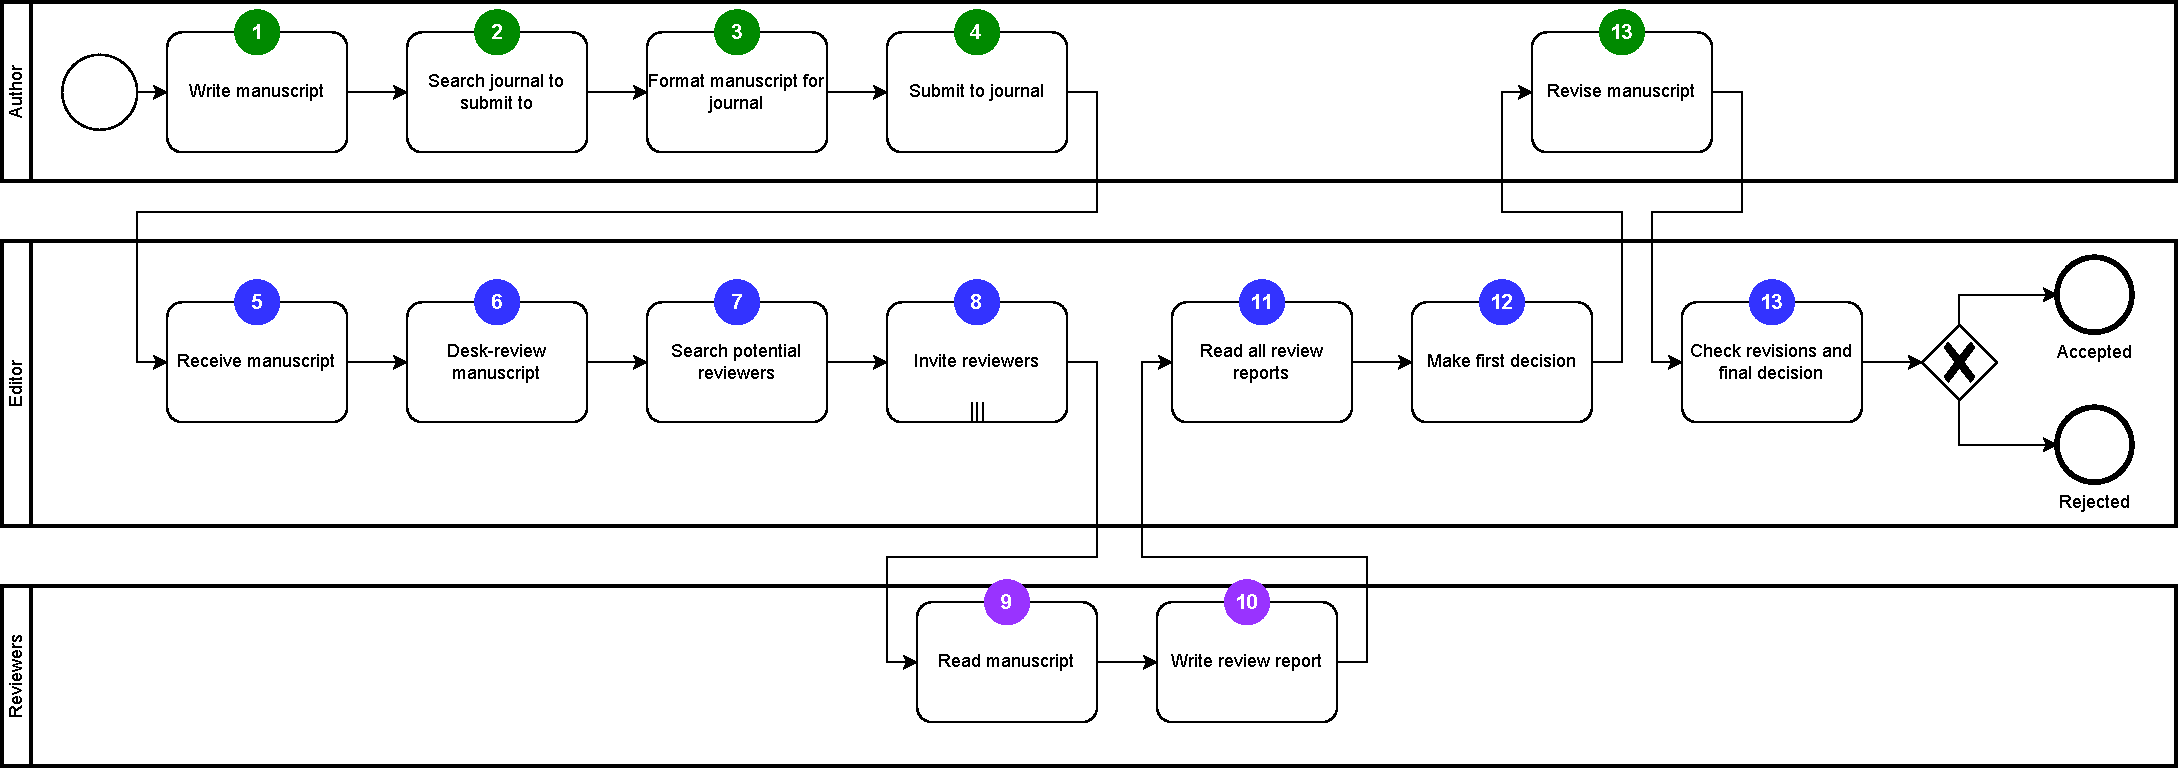
\includegraphics[width=\linewidth]{editorial_process.pdf}
    \end{figure*}
\end{landscape}


